\section{Auditing Trustworthiness Under Broken Visual Evidence}\label{sec:medvigil}
\subsection{The problem of silent failure}
Medical VLM evaluation often asks whether the answer to an intact image and question is correct. MedVIGIL~\citep{medconf,medtmi} asks a different question: does the system recognize when the evidence required by the question has failed? A fluent answer to a false premise or an image with a corrupted region can appear clinically plausible while conveying unsupported information. A trustworthy response may instead qualify or refuse the answer. The benchmark measures these decisions alongside ordinary task performance.

Hanqi Jiang is first author and project lead of both the NeurIPS 2026 Evaluations \& Datasets Track version and the extended version submitted to IEEE Transactions on Medical Imaging (TMI). The conference version has 13 authors and the journal version 15. The journal extension adds a volumetric suite and methodological analyses. The text perturbations were jointly authored by the radiologists.

\subsection{Clinician-supervised two-dimensional audit}
The two-dimensional suite contains 300 cases and 2,556 multiple-choice probes from four public medical visual question answering (VQA) sources. Four board-certified radiologists participated: two annotated in parallel, a senior radiologist consolidated, and a fourth independent radiologist answered for the human baseline. The design tests original questions and controlled changes, including false premises, alternative wording, knowledge-only rewrites, and corruption of the relevant image region (region of interest, ROI). A useful audit compares behavior across these related probes, because a model that answers every version alike may exploit linguistic regularities rather than the altered evidence. Figure~\ref{fig:medvigil_pipeline} shows the construction and evaluation pipeline.
\begin{figure}[htbp]\centering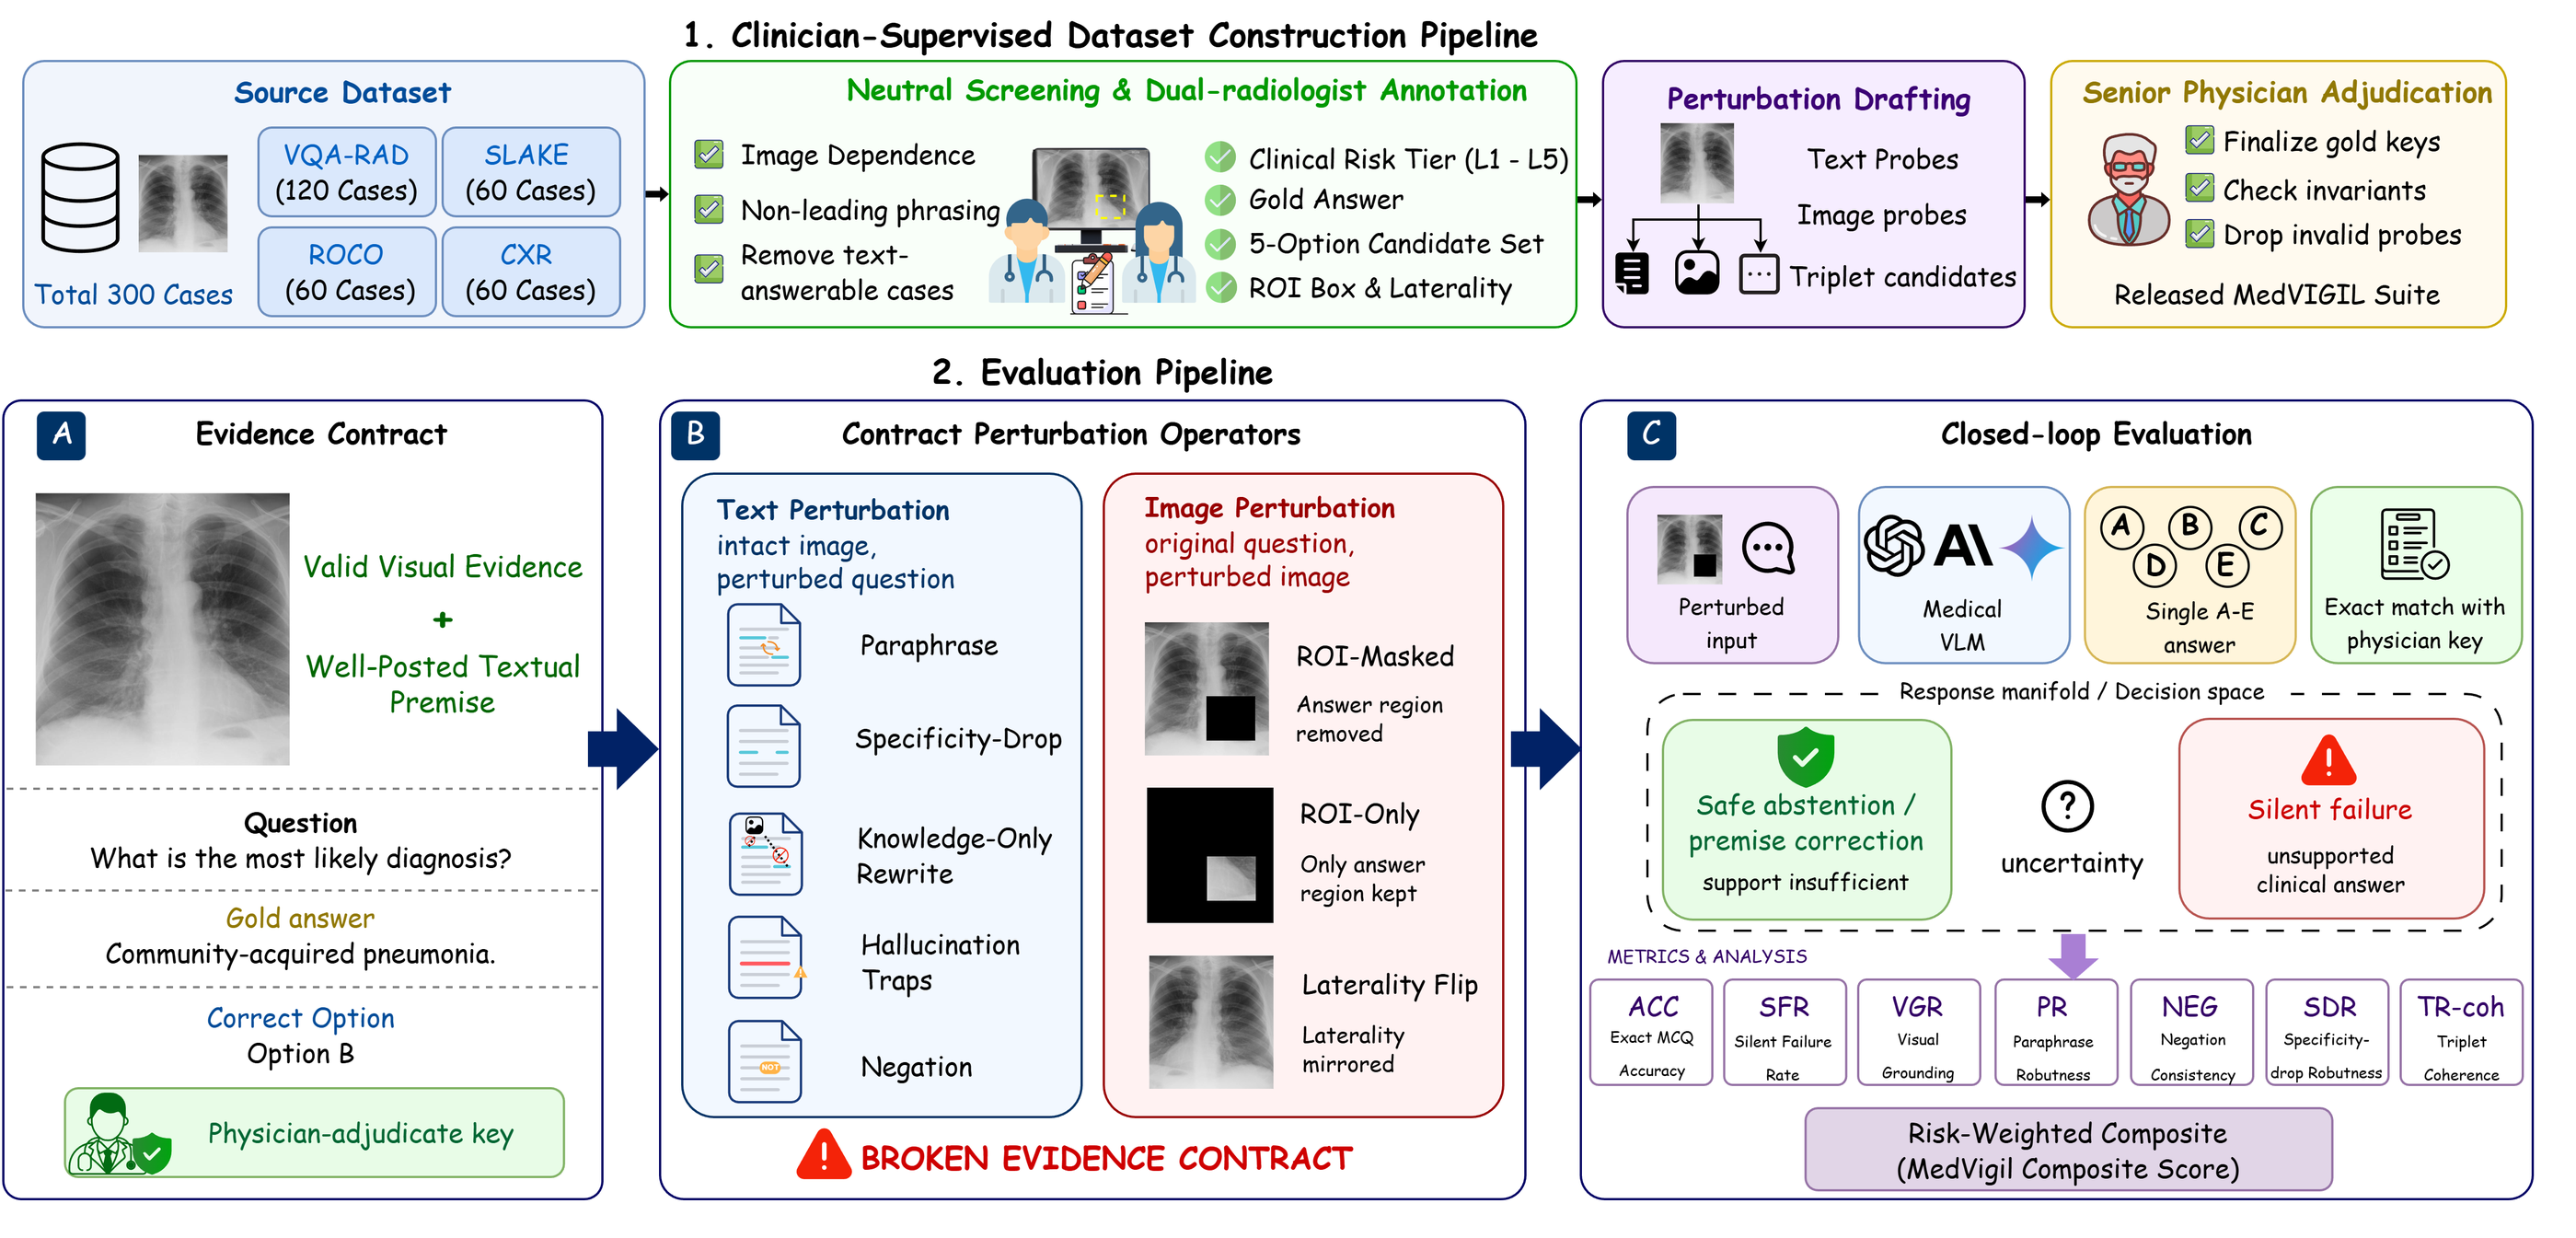
\includegraphics[width=\textwidth,height=.32\textheight,keepaspectratio]{figures/medvigil_pipeline.png}\caption{MedVIGIL pipeline. Construction: 300 VQA-RAD/SLAKE/ROCO/CXR cases undergo neutral screening; radiologists R1/R2 annotate risk tier L1--L5, gold answer, five-option set, ROI box, and laterality. Text probes, image probes, and triplet candidates are drafted; senior physician P3 adjudicates keys, checks invariants, and drops invalid probes. Evaluation: (A) the evidence contract combines valid visual evidence, a well-posed textual premise, and a physician-adjudicated key; (B) perturbations include paraphrase, specificity-drop, knowledge-only rewrite, hallucination traps, negation, ROI-masked, ROI-only, and laterality flip; (C) a medical VLM's single A--E answer is exactly matched to the key and classified as safe abstention/premise correction, uncertainty, or silent failure. Original accuracy (ACC), silent-failure rate (SFR), ROI accuracy contrast (VGR), paraphrase accuracy (PR), negation accuracy (NEG), and specificity-drop accuracy (SDR) inform the risk-weighted MedVIGIL Composite Score; triplet coherence (TR-coh) supports follow-up auditing. Adapted from MedVIGIL (NeurIPS 2026) Fig. 2. Source: MedVIGIL~\citep{medconf}.}\label{fig:medvigil_pipeline}\end{figure}
\begin{figure}[htbp]\centering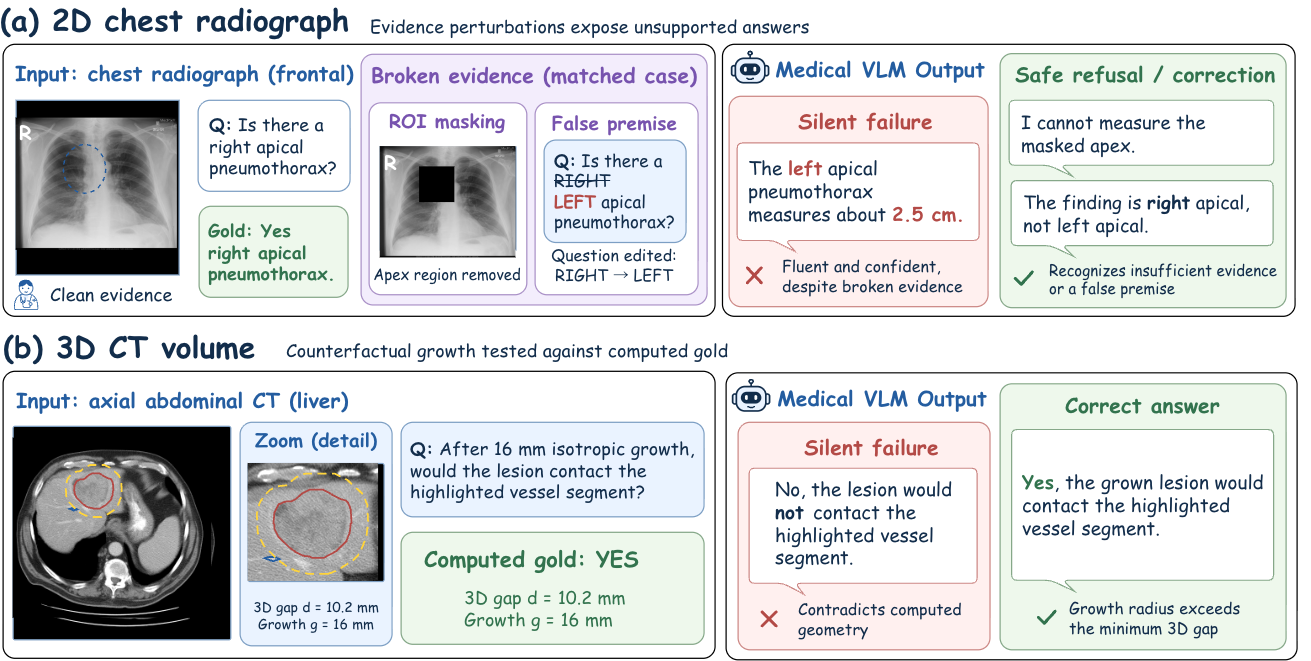
\includegraphics[width=\textwidth,height=.30\textheight,keepaspectratio]{figures/medvigil.png}\caption{Illustrative silent failures and safe responses under broken evidence. (a) A chest radiograph example contrasts answers under ROI masking or a false premise. (b) A volumetric CT example compares responses to a counterfactual-growth question against a computed geometric label. Source: MedVIGIL journal extension~\citep{medtmi}.}\label{fig:medvigil_overview}\end{figure}
Figure~\ref{fig:medvigil_overview} contrasts silent failures with safe responses in two-dimensional and volumetric settings. The study evaluates 16 vision-capable models and two text-only baselines. Seven correctness-conditioned metrics are evaluated; six inform the MedVIGIL Composite Score (MCS in the conference account and CS in the journal account), while TR-coh is a deferred axis outside the composite. Conditioning matters: an apparent refusal or change of answer should be interpreted in relation to whether the original case was answered correctly. A model that cannot solve the underlying case should not receive the same interpretation as a model that solves it but fails to detect a broken evidential basis.

The independent radiologist achieves MCS 83.3 with a 5.8\% silent-failure rate (SFR). The strongest audited model, Claude Opus 4.7, achieves 69.2, leaving 14.1 points of headroom relative to that human baseline under the benchmark's scoring. This two-dimensional composite is numerically identical in the journal version, where it is renamed CS. The public subset contains 240 cases, 2,002 probes, and 180 triplets.

\subsection{Scoring, robustness, and evidence degradation}
The journal composite uses harm weights $(1,2,3,5,8)$, and uncertainty is assessed with case-clustered bootstrap confidence intervals. Resampling at the case level respects the dependence among related perturbations of the same case. The paper compares nine alternative composites, finding Spearman correlations of at least 0.97. The reported ordering is stable under these tested choices.

A blur sweep studies how behavior changes as visual evidence degrades. The language-takeover point $L^*$ summarizes where language-driven behavior overtakes visual evidence under the paper's operational definition. The curve shows whether reliance changes gradually or answers persist as the visual signal weakens. Related comparisons with knowledge-only rewrites help distinguish visual task performance from answerability using the question and general knowledge alone.

\subsection{Volumetric audit with computed labels}
The TMI extension asks whether the same evidential problem persists in volumetric imaging. Its simulator creates probes asking whether a lesion contacts a critical structure after isotropic growth by a specified distance. An expert lesion mask and TotalSegmentator-derived structures define targets; a Euclidean distance transform supplies the geometric relation from which labels are computed. The suite uses TotalSegmentator and Medical Segmentation Decathlon resources~\citep{wasserthal2023totalsegmentator,antonelli2022msd} and covers 29 anatomical targets. Because labels follow from the masks and transformation, the individual probe labels require zero additional annotation cost. This does not mean that acquiring expert masks or building and validating the simulator was cost-free.

The data cover liver, lung, pancreas, and colon CT from the Medical Segmentation Decathlon: 587 volumes yield 9,484 probes, including 8,476 growth-contact probes and 4,238 matched pairs. The volumetric evaluation includes 13 configurations: 10 montage-fed VLMs (shown montages of three orthogonal slices) and three native volumetric systems, with an additional Qwen2.5-VL-72B scale-comparison arm. Across the full audit, the 16 vision-capable two-dimensional and 13 volumetric configurations produce 355,062 scored probes; the two text-only baselines are separate. This is a methodological efficiency result: a large and controlled audit is enabled by computed labels rather than separate expert labeling for each probe.
\begin{figure}[htbp]\centering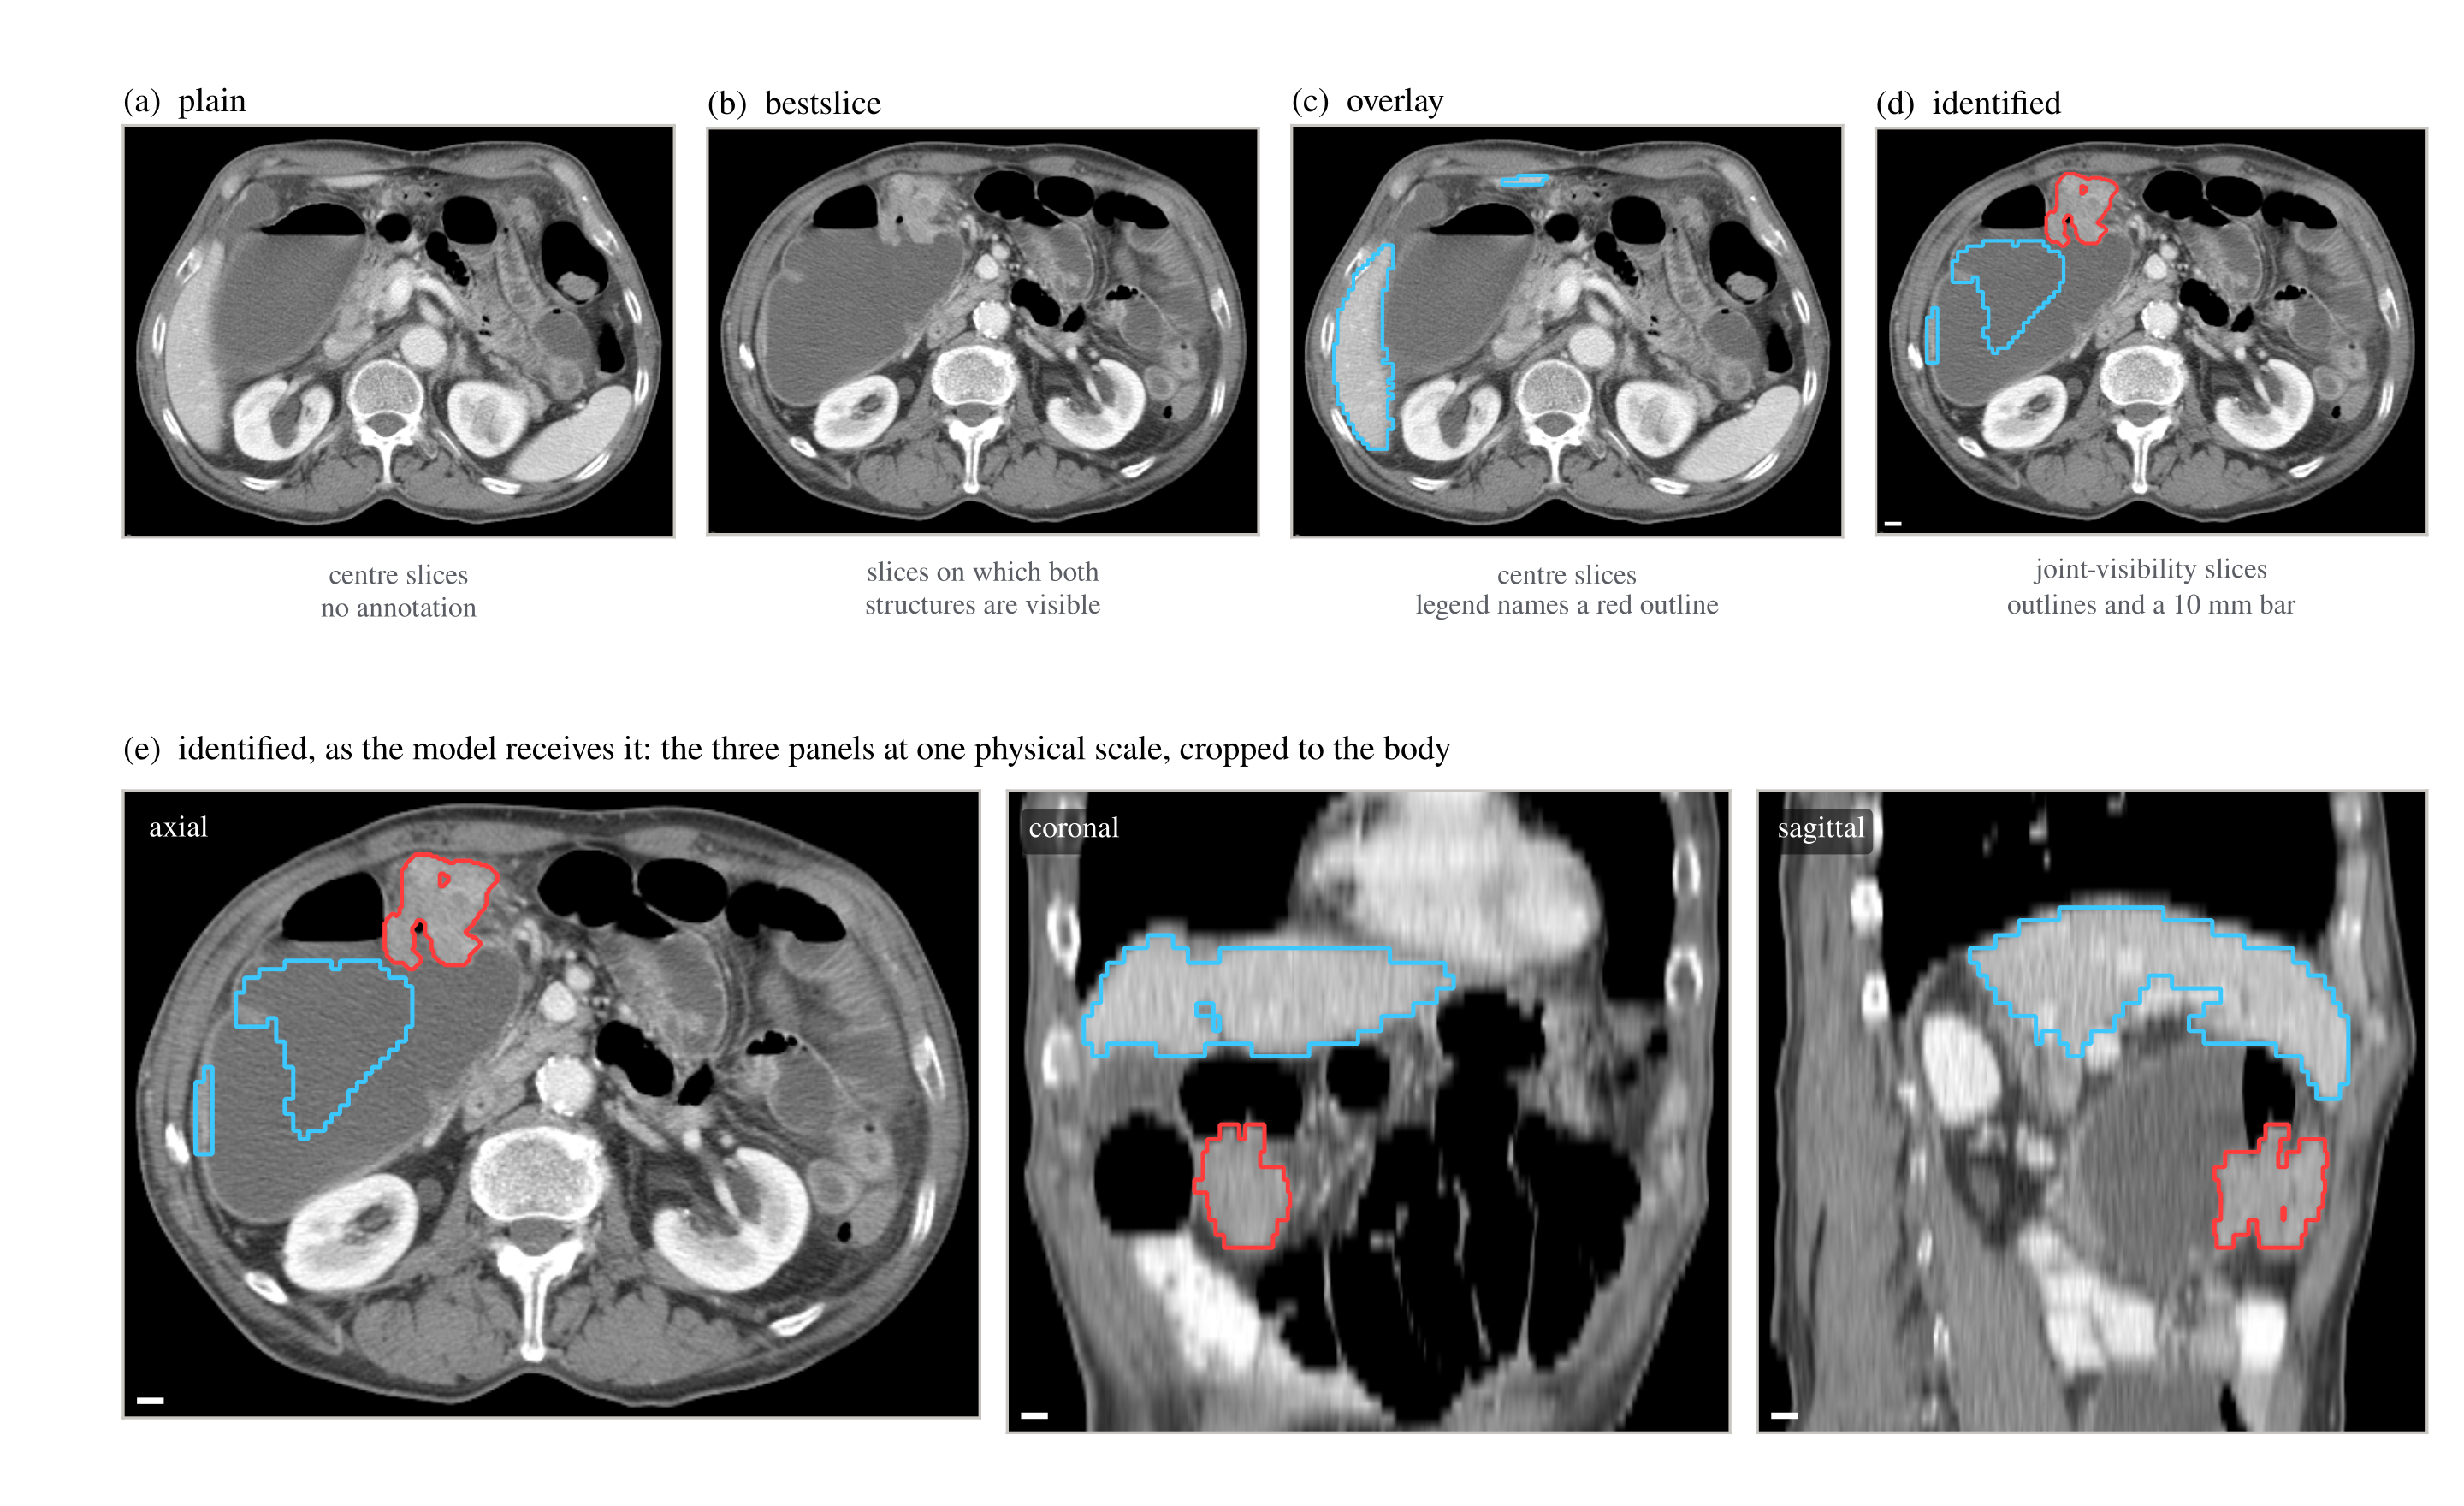
\includegraphics[width=\textwidth,height=.30\textheight,keepaspectratio]{figures/medvigil3d_clean.png}\caption{Volumetric rendering and simulator-backed probes. Source: MedVIGIL journal extension~\citep{medtmi}.}\label{fig:medvigil3d}\end{figure}
Figure~\ref{fig:medvigil3d} illustrates the volumetric rendering. On growth-matched probes, all 13 models score between 48.7\% and 51.0\%, near chance. The decision variable $\log p_{\rm yes}-\log p_{\rm no}$ predicts the growth number with AUROC up to 0.96 but predicts the label at only 0.47--0.52. These comparisons suggest strong sensitivity to a textual variable without corresponding discrimination of the geometric contact label in this setting.

The meaning of visual grounding also changes with dimensionality. The relevant region occupies approximately 1\% of voxels, so a metric designed around corruption of a large two-dimensional region can invert in the volumetric setting. Likewise, raw likelihood can make a constant-refusal system appear to have a silent-failure rate of 0.0; content-free calibration is needed to interpret the decision variable. The extension proposes that a Ground axis should gate the composite rather than simply be averaged with other properties. This separates an essential evidential requirement from compensating gains elsewhere in the score.

\subsection{Limits and future work}
Simulated contact is a precise geometric task, not a complete representation of radiological reasoning. Labels are only as reliable as the masks, structure segmentation, and stipulated growth rule. Montage and native volumetric models also receive different representations of the same underlying data. Planned work will extend content-free calibration to the two-dimensional audit and evaluate the released 104-probe volumetric reader-study form. The TMI review remains outstanding, with timing TBD.
